\documentclass[aspectratio=169,9pt]{beamer}

% ── Thème ──
\usetheme{Madrid}
\usefonttheme{professionalfonts}

% ── Packages ──
\usepackage[utf8]{inputenc}
\usepackage[T1]{fontenc}
\usepackage[french]{babel}
\usepackage{lmodern}
\usepackage{amsmath,amssymb}
\usepackage{graphicx}
\usepackage{booktabs}
\usepackage{xcolor}
\usepackage{colortbl}
\usepackage{array}
\usepackage{microtype}
\usepackage{tikz}
\usetikzlibrary{calc}

% ── Charte UTC ──
\definecolor{UTCYellow}{RGB}{252,192,0}
\definecolor{UTCGray}{RGB}{72,72,72}
\definecolor{UTCLightGray}{RGB}{130,130,130}
\definecolor{RedUTC}{RGB}{190,30,45}
\definecolor{RiskHL}{RGB}{255,210,210}
\definecolor{GreenHL}{RGB}{215,242,215}
\definecolor{YellowHL}{RGB}{255,248,195}

% ── Palette Beamer ──
\setbeamercolor{palette primary}{bg=UTCYellow,fg=UTCGray}
\setbeamercolor{palette secondary}{bg=UTCGray,fg=white}
\setbeamercolor{palette tertiary}{bg=UTCLightGray,fg=white}
\setbeamercolor{palette quaternary}{bg=UTCGray!85!black,fg=white}
\setbeamercolor{structure}{fg=UTCGray}
\setbeamercolor{frametitle}{bg=UTCGray,fg=white}
\setbeamercolor{title}{fg=UTCGray}
\setbeamercolor{subtitle}{fg=UTCGray!75!black}
\setbeamercolor{author}{fg=UTCGray}
\setbeamercolor{institute}{fg=UTCGray!80!black}
\setbeamercolor{date}{fg=UTCGray!80!black}
\setbeamercolor{block title}{bg=UTCGray,fg=white}
\setbeamercolor{block body}{bg=UTCGray!7!white}
\setbeamercolor{block title alerted}{bg=RedUTC,fg=white}
\setbeamercolor{block body alerted}{bg=RedUTC!7!white}
\setbeamercolor{block title example}{bg=UTCYellow,fg=UTCGray}
\setbeamercolor{block body example}{bg=YellowHL}
\setbeamercolor{alerted text}{fg=RedUTC}

% ── Filet jaune sous le titre de chaque slide (via beamercolorbox) ──
\addtobeamertemplate{frametitle}{}{%
  \nointerlineskip%
  \begin{beamercolorbox}[wd=\paperwidth,ht=1.8pt,dp=0pt]{palette primary}%
  \end{beamercolorbox}%
}

% ── Pied de page ──
\setbeamertemplate{footline}{%
  \leavevmode\hbox{%
    \begin{beamercolorbox}[wd=.30\paperwidth,ht=2.25ex,dp=1ex,center]{palette secondary}
      \usebeamerfont{author in head/foot}\insertshortauthor
    \end{beamercolorbox}%
    \begin{beamercolorbox}[wd=.45\paperwidth,ht=2.25ex,dp=1ex,center]{palette tertiary}
      \usebeamerfont{title in head/foot}\insertshorttitle
    \end{beamercolorbox}%
    \begin{beamercolorbox}[wd=.25\paperwidth,ht=2.25ex,dp=1ex,right]{palette primary}
      \usebeamerfont{date in head/foot}%
      \textcolor{UTCGray}{\insertshortdate\hspace*{1.2em}%
      \insertframenumber{}\,/\,\inserttotalframenumber\hspace*{1ex}}%
    \end{beamercolorbox}%
  }%
}

% ── Métadonnées ──
\title[Décrochage scolaire en mathématiques]{%
  Identification des profils à risque de décrochage en mathématiques}
\subtitle{Distance de Gower · AFTD · Clustering · Apprentissage supervisé}
\author[Gros · Lozac'h · Piekarz]{%
  Mathéo Gros \quad Maël Lozac'h \quad Mathieu Piekarz}
\institute[UTC : SY09]{%
  Université de Technologie de Compiègne \quad SY09 : Sciences des Données}
\date{P26}

\newcommand{\code}[1]{\texttt{\small #1}}

% ════════════════════════════════════════════════════════
\begin{document}
% ════════════════════════════════════════════════════════

% ── Page de titre : fond pleine page via TikZ ──
{%
\usebackgroundtemplate{%
  \begin{tikzpicture}[remember picture,overlay]
    % Bande jaune en haut (plein bord)
    \fill[UTCYellow]
      (current page.north west) rectangle
      ($(current page.north east)+(0,-1.3cm)$);
    % Filet jaune au-dessus de la zone grise
    \fill[UTCYellow]
      ($(current page.south west)+(0,2.1cm)$) rectangle
      ($(current page.south east)+(0,2.13cm)$);
    % Bande grise en bas (plein bord)
    \fill[UTCGray]
      (current page.south west) rectangle
      ($(current page.south east)+(0,2.1cm)$);
  \end{tikzpicture}%
}%
\begin{frame}[plain,noframenumbering]
  \begin{tikzpicture}[remember picture,overlay]
    % Logo UTC (dans la bande jaune, aligné à droite)
    \node[anchor=north east, inner sep=0.17cm]
      at ($(current page.north east)+(0,-0.08cm)$)
      {
\includegraphics[height=0.95cm]{../figures/UTCLOGO.png}};
    % Titre (centré dans la zone blanche)
    \node[anchor=center, text width=0.88\paperwidth, align=center]
      at ($(current page.center)+(0,0.55cm)$)
      {{\fontsize{18}{22}\selectfont\bfseries\color{UTCGray}
      SY09 - Sciences des Données\\[4pt]
        Identification des profils à risque\\[1pt]
        de décrochage en mathématiques}};
    % Bloc auteurs / info (dans la bande grise)
    \node[anchor=north, text width=0.95\paperwidth, align=center]
      at ($(current page.south)+(0,2.08cm)$)
      {%
        \vspace{0.28cm}%
        {\normalsize\bfseries\color{white}
          Mathéo Gros
          \enspace{\color{UTCYellow}|}\enspace
          Maël Lozac'h
          \enspace{\color{UTCYellow}|}\enspace
          Mathieu Piekarz}\\[0.16cm]
        {\footnotesize\color{white!82!UTCGray}
          Université de Technologie de Compiègne
          \enspace\textbullet\enspace
          SY09 Sciences des Données
          \enspace\textbullet\enspace
          P26}\\[0.10cm]
        {\footnotesize\color{white!65!UTCGray}
          G.~Govaert
          \enspace{\color{UTCYellow}|}\enspace
          T.~Denœux
          \enspace{\color{UTCYellow}|}\enspace
          B.~Quost
          \enspace{\color{UTCYellow}|}\enspace
          S.~Rousseau}%
      };
  \end{tikzpicture}
\end{frame}
}%

% ────────────────────────────────────────────────────────
%  MINUTE 1 : Slide 1 : Contexte
% ────────────────────────────────────────────────────────
\begin{frame}{Contexte : un écart statistiquement significatif}
\begin{columns}[c]
  \column{0.43\textwidth}
    \begin{block}{Données : UCI Student Dataset}
      \footnotesize
      \begin{itemize}\setlength\itemsep{1pt}
        \item \textbf{395 élèves} de lycée portugais
        \item Variables socio-familiales et comportementales\\
              disponibles \emph{avant les résultats finaux}
        \item Deux matières : mathématiques \& portugais
      \end{itemize}
    \end{block}
    \vspace{2pt}
    \begin{alertblock}{Définition : Décrocheur}
      \footnotesize
      $\delta_i = \mathbf{1}\bigl[(G_3 = 0) \cap (G_1 > 0)\bigr]$\\[2pt]
      Signal de départ \emph{en cours d'année} (distinct de l'absence initiale).
    \end{alertblock}
    \vspace{2pt}
    \begin{exampleblock}{Asymétrie observée ($\chi^2$, $p < 0{,}001$)}
      \footnotesize\centering
      \renewcommand{\arraystretch}{1.05}
      \begin{tabular}{lcc}
        \toprule
                           & Maths            & Portugais \\
        \midrule
        Taux décrochage    & \textbf{9,6\,\%} & 2,3\,\%   \\
        Effectif           & \textbf{38}       & 13        \\
        \bottomrule
      \end{tabular}\\[2pt]
      Signal propre aux mathématiques.
    \end{exampleblock}
    \vspace{1pt}
    {\scriptsize\itshape\centering$\hookrightarrow$Objectif : détecter ces élèves \emph{avant} la fin d'année, via les seules variables de rentrée.\par}

  \column{0.54\textwidth}
    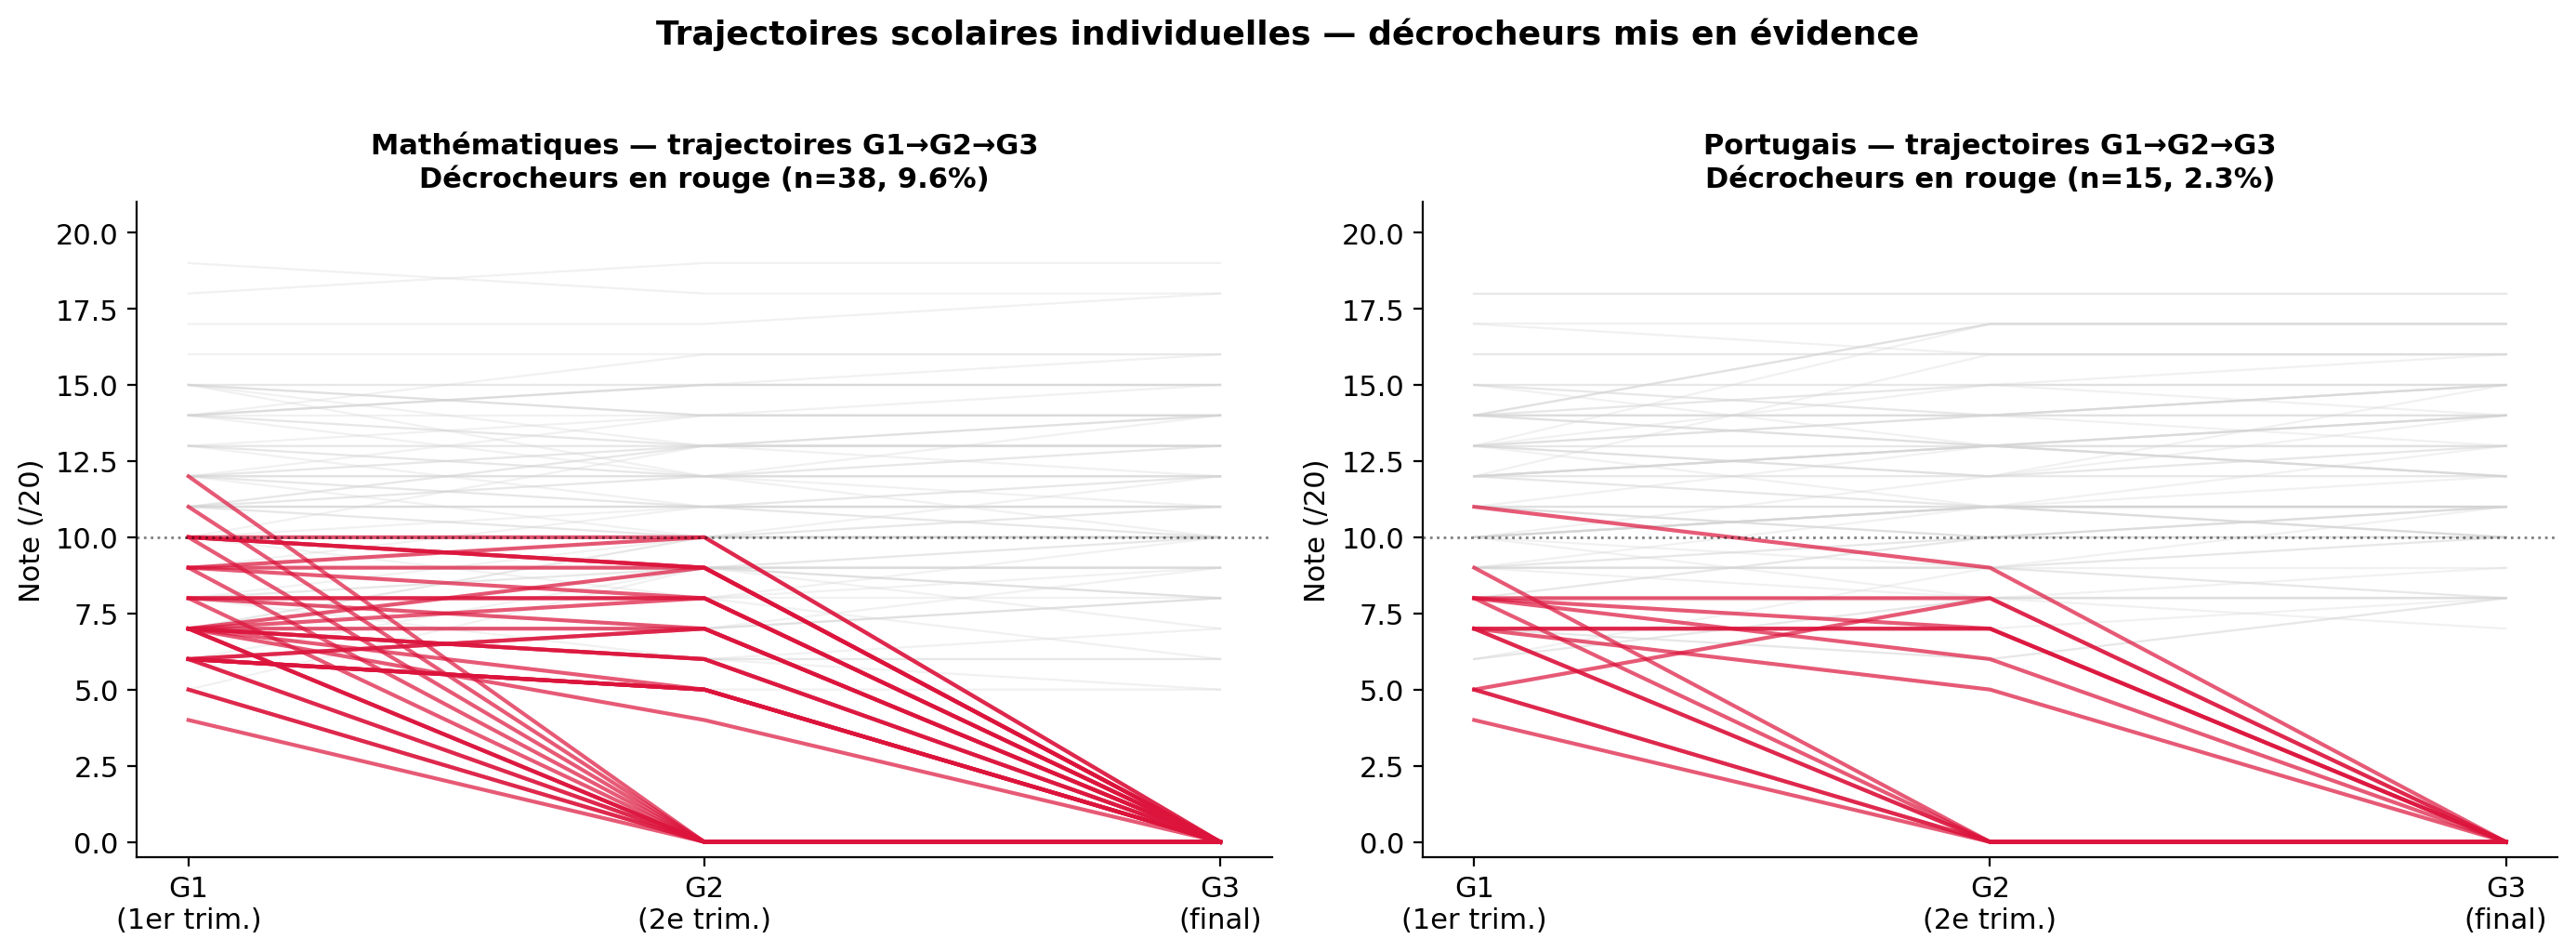
\includegraphics[width=\linewidth]{../figures/00_trajectoires_decrochage.png}
\end{columns}
\end{frame}

% ────────────────────────────────────────────────────────
%  MINUTE 1 : Slide 2 : Problématique & Variables
% ────────────────────────────────────────────────────────
\begin{frame}{Problématique et sélection des variables}
\begin{center}
  \fcolorbox{UTCYellow}{YellowHL}{\parbox{0.88\textwidth}{%
    \centering\itshape\footnotesize
    \textbf{Dans quelle mesure} les variables socio-comportementales disponibles en début d'année
    permettent-elles d'\textbf{identifier les profils d'élèves susceptibles de décrocher en mathématiques}?
  }}
\end{center}
\vspace{3pt}
\begin{columns}[c]
  \column{0.35\textwidth}
    \begin{block}{8 variables retenues ($\alpha = 0{,}10$)}
      \footnotesize\centering
      \renewcommand{\arraystretch}{1.05}
      \begin{tabular}{ll}
        \toprule
        \textbf{Numériques} & \textbf{Catégorielles} \\
        \midrule
        \code{failures}     & \code{higher}     \\
        \code{Medu}         & \code{paid}       \\
        \code{age}          & \code{schoolsup}  \\
        \code{Walc}         & \code{romantic}   \\
        \bottomrule
      \end{tabular}\\[-1pt]
      {\scriptsize\itshape Tests : Mann-Whitney (num.) · $\chi^2$ (cat.)}
    \end{block}
    \vspace{3pt}
    {\footnotesize\textcolor{RedUTC}{\textbf{Exclusion \code{absences} :}}
    paradoxe : les décrocheurs ont \emph{0 absence} enregistrée (artefact post-départ).}

  \column{0.62\textwidth}
    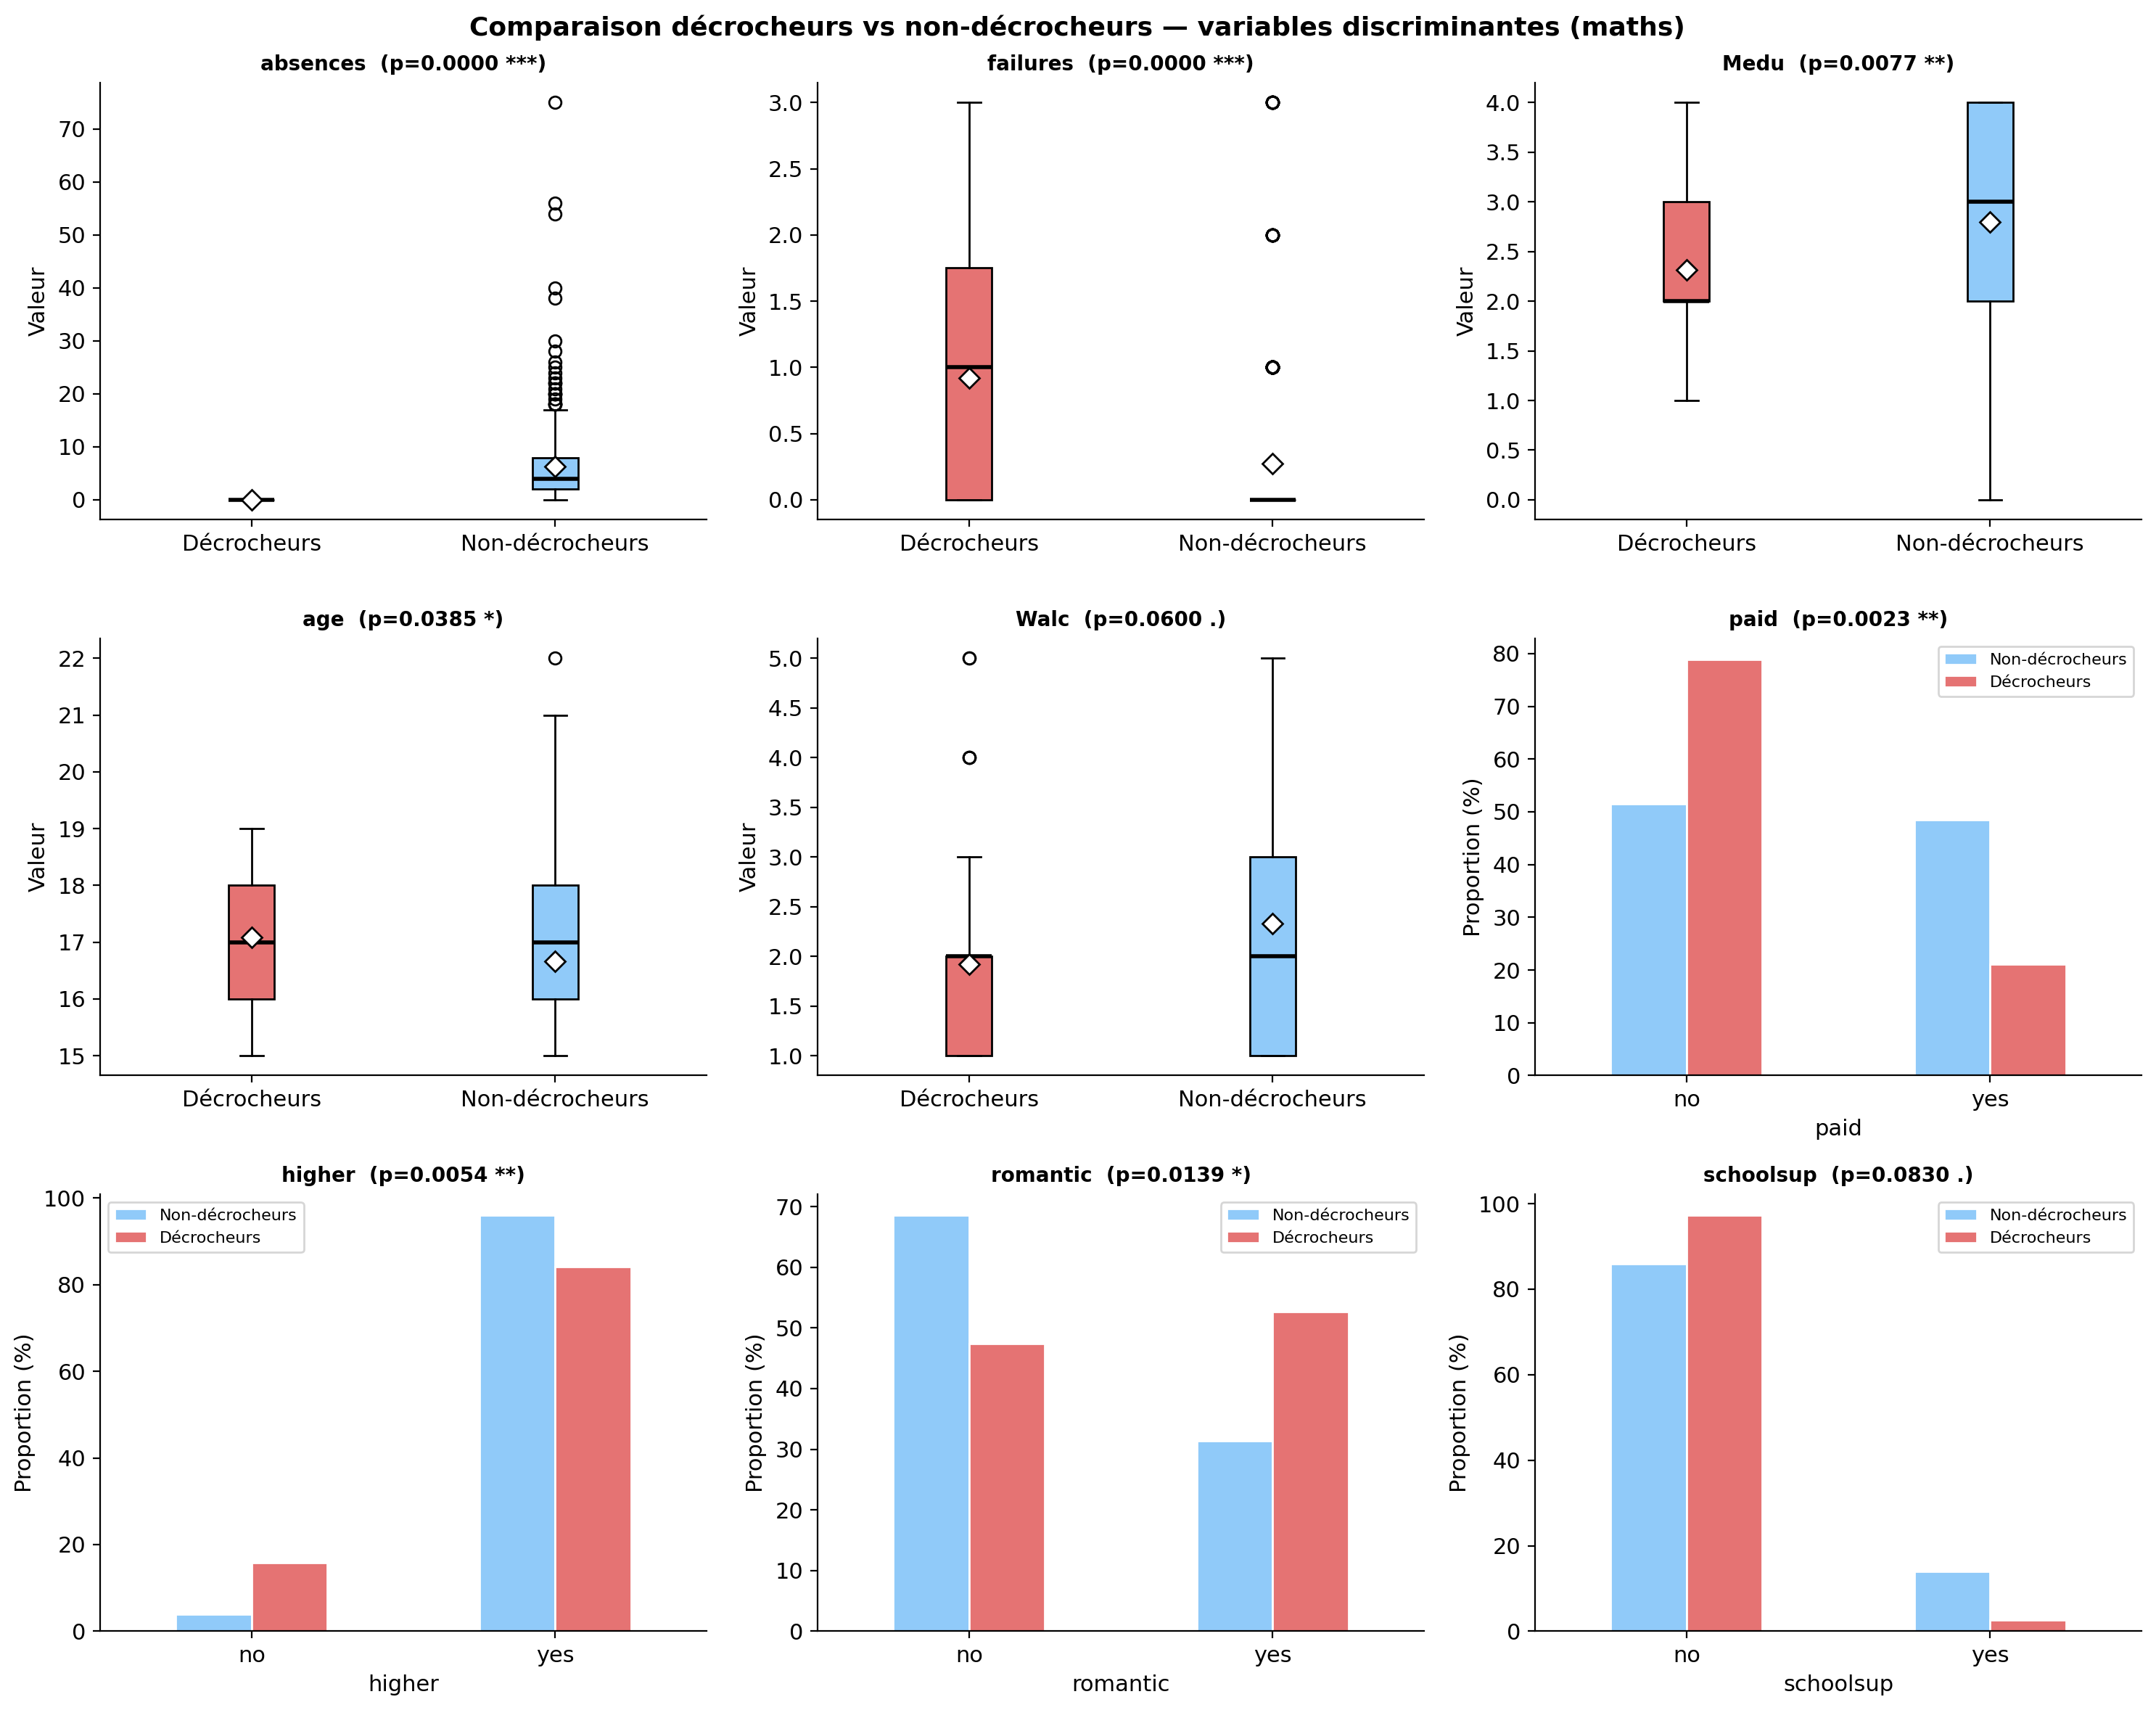
\includegraphics[width=0.88\linewidth]{../figures/00_discriminants.png}
\end{columns}
\end{frame}

% ────────────────────────────────────────────────────────
%  MINUTE 2 : Slide 3 : Distance de Gower + AFTD
% ────────────────────────────────────────────────────────
\begin{frame}{Réduction dimensionnelle : distance de Gower et AFTD}
\begin{columns}[c]
  \column{0.42\textwidth}
    \begin{block}{Distance de Gower : variables hétérogènes}
      \footnotesize
      Pour $p$ variables, entre individus $i$ et $j$ :
      $$d_{ij} = \frac{1}{p}\sum_{k=1}^{p}\delta_{ij}^{(k)}$$
      \vspace{-6pt}
      \begin{itemize}\setlength\itemsep{1pt}
        \item Ordinale : $\delta^{(k)} = |x_i^{(k)}-x_j^{(k)}|\,/\,r_k$
        \item Binaire  : $\delta^{(k)} = \mathbf{1}[x_i^{(k)}\neq x_j^{(k)}]$
      \end{itemize}
      {\scriptsize\itshape$\hookrightarrow$Euclidienne inadaptée aux variables mixtes num./cat.}
    \end{block}
    \vspace{3pt}
    \begin{block}{AFTD : Analyse Factorielle des Distances}
      \footnotesize
      Double centrage de $\Delta^2$ :
      $$W = -\tfrac{1}{2}\,Q_n\Delta^2 Q_n,\quad
        Q_n = I_n - \tfrac{\mathbf{1}\mathbf{1}^\top}{n}$$
      \vspace{-4pt}
      Décomposition spectrale $W=U\Lambda U^\top$
      $\;\Rightarrow\;$ coordonnées $C = U_+\Lambda_+^{1/2}$\\
      {\scriptsize\itshape$\hookrightarrow$L'ACP requiert des variables brutes ; l'AFTD opère directement sur $\Delta$.}
    \end{block}

  \column{0.55\textwidth}
    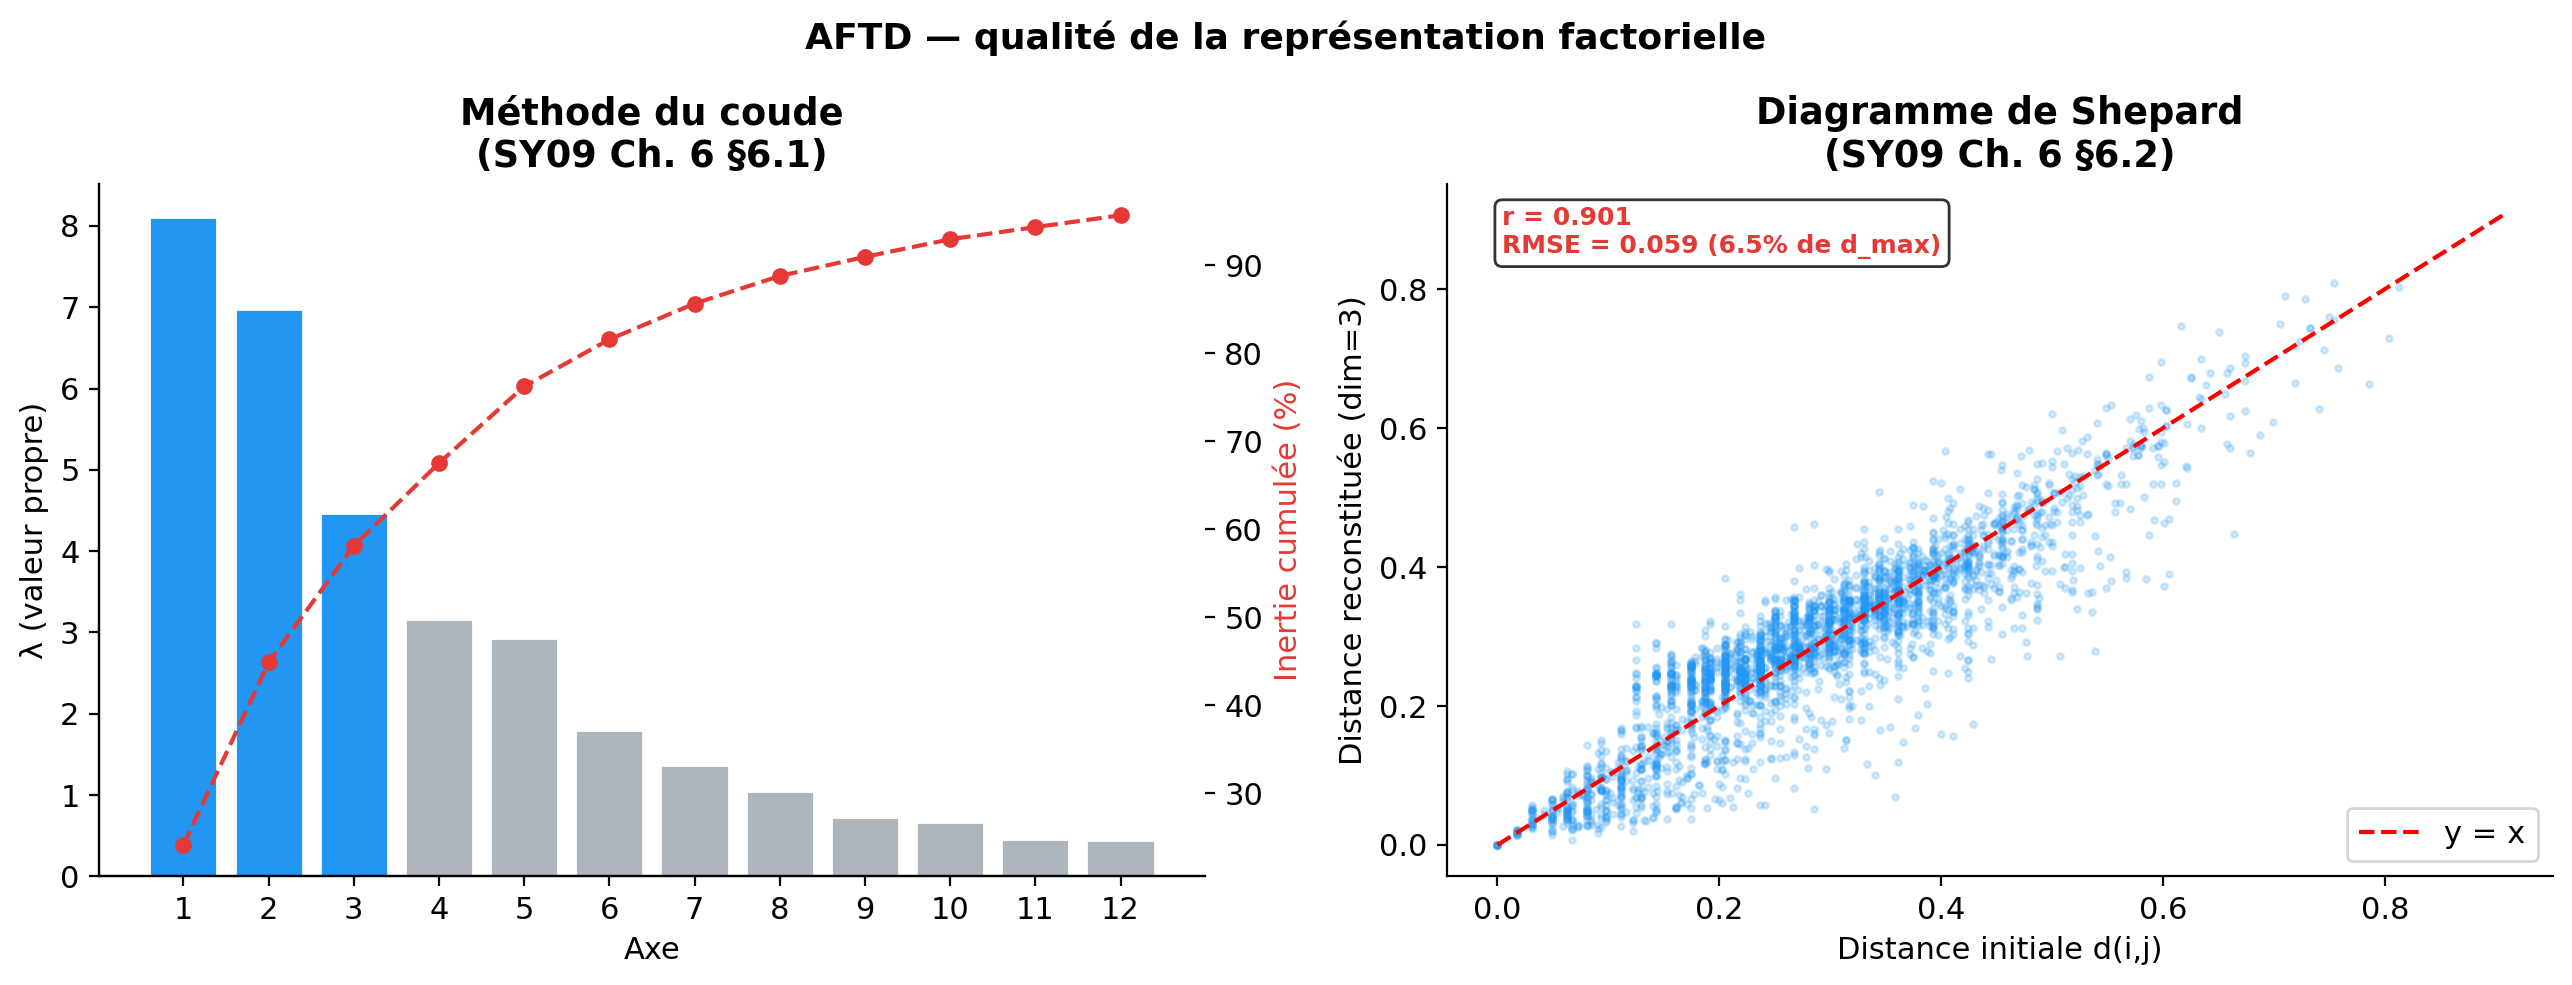
\includegraphics[width=\linewidth]{../figures/03_aftd_scree_shepard.png}\\[2pt]
    \centering{\footnotesize
      \textbf{2 axes} · 44,9\,\% inertie ·
      Shepard $r=0{,}90$ · RMSE $=6{,}5\,\%\,d_\mathrm{max}$
    }
\end{columns}
\end{frame}

% ────────────────────────────────────────────────────────
%  MINUTE 2 : Slide 4 : Clustering K = 4
% ────────────────────────────────────────────────────────
\begin{frame}{Clustering : 4 profils robustes : ARI\,=\,1,000}
\begin{columns}[c]
  \column{0.50\textwidth}
    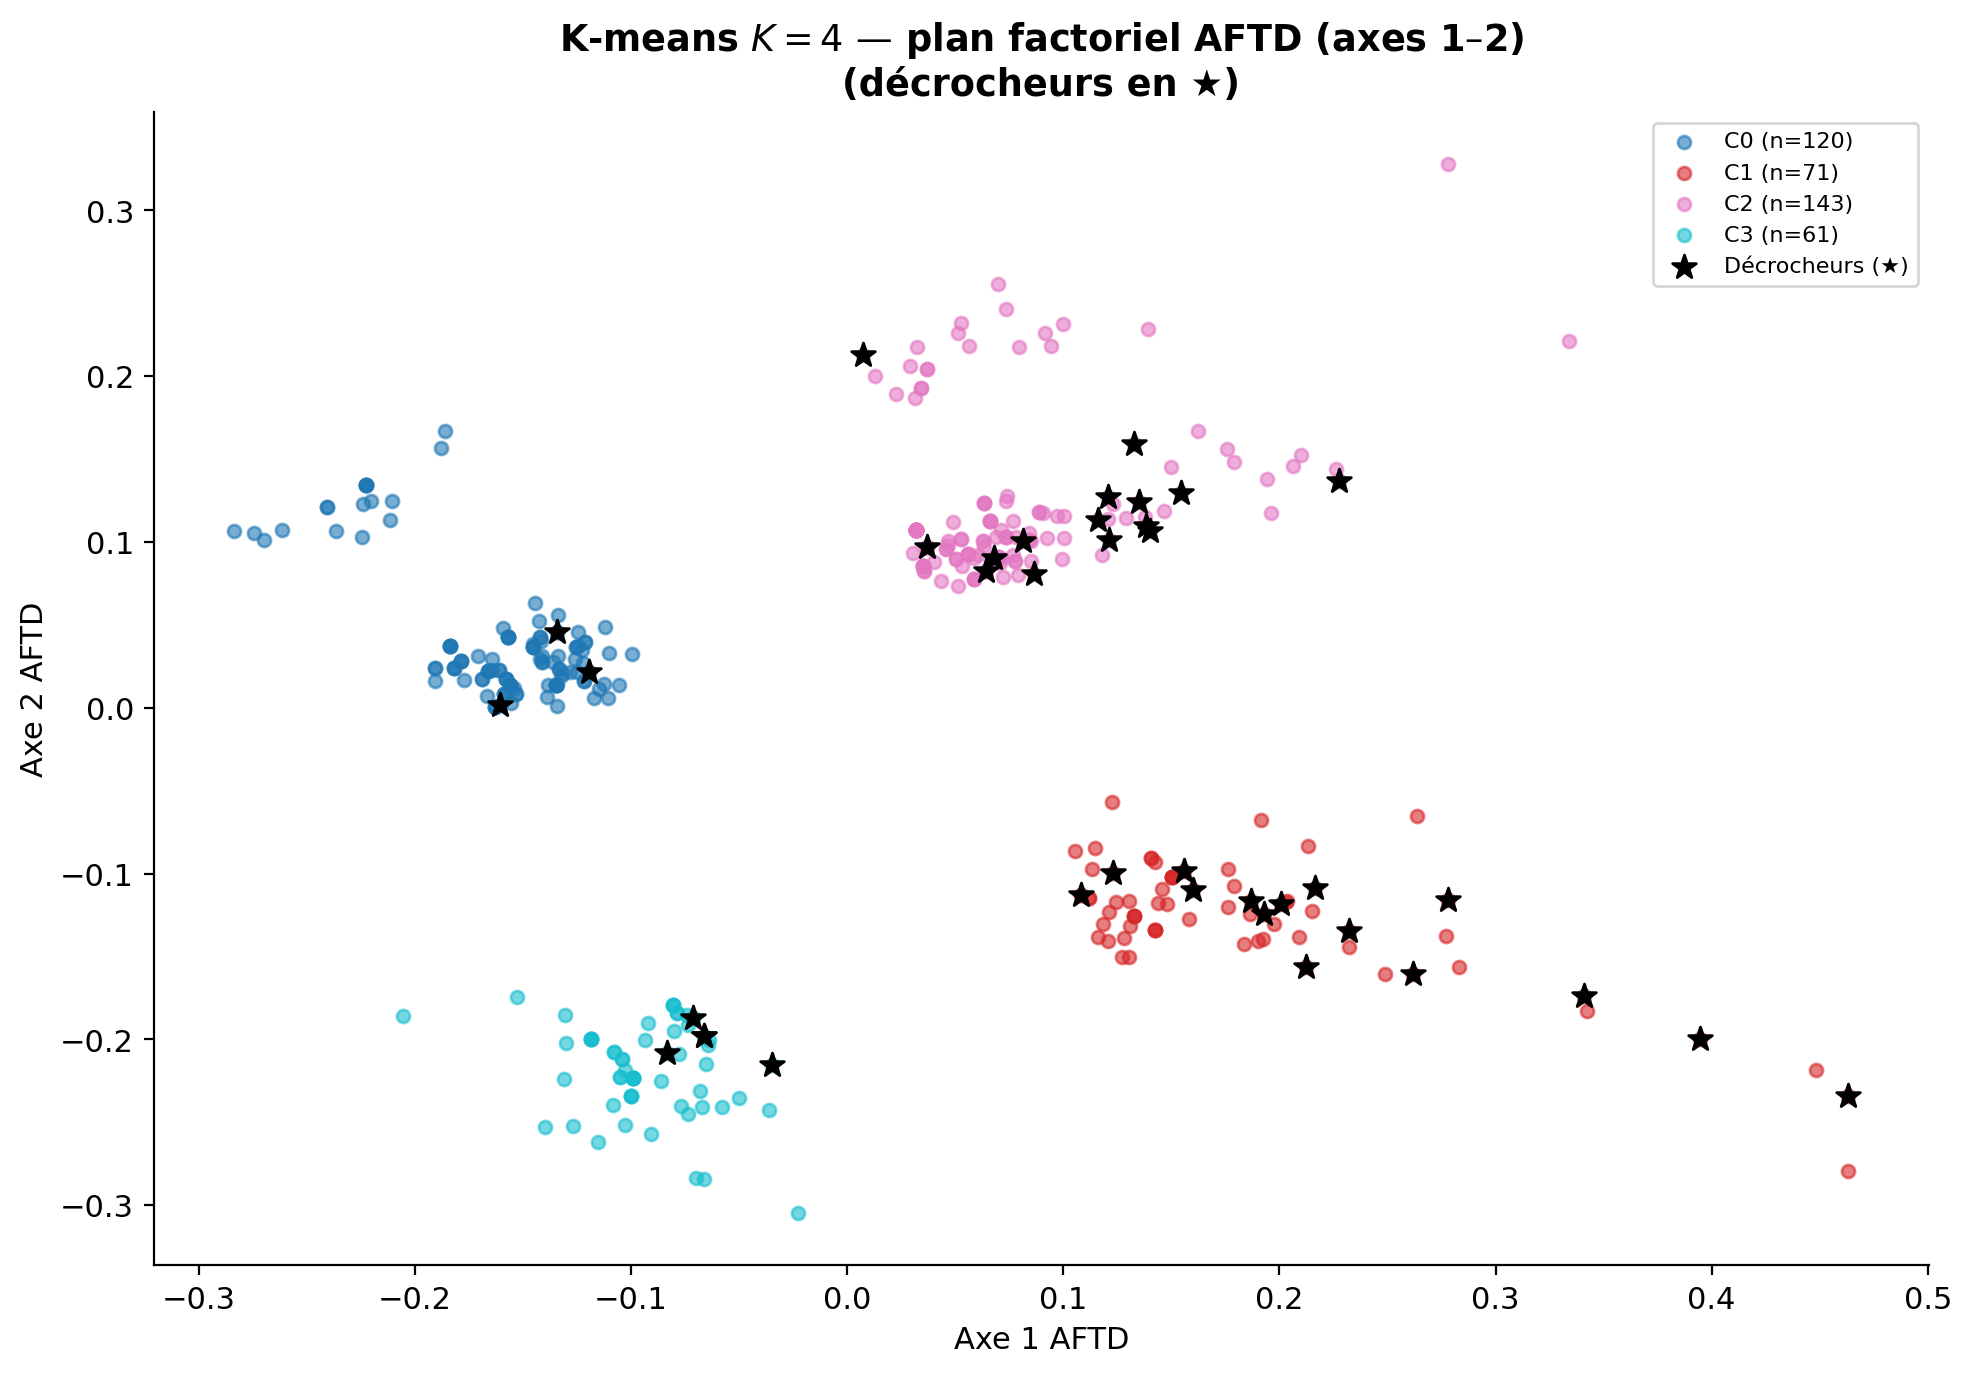
\includegraphics[width=\linewidth]{../figures/03_plan_factoriel_clusters.png}

  \column{0.47\textwidth}
    \begin{alertblock}{Convergence CAH-Ward / K-means}
      \footnotesize\centering
      $\mathrm{ARI}=1{,}000\;\Rightarrow$ \textbf{partitions identiques}\\
      Résultat robuste, indépendant de la méthode.\\
      {\scriptsize\itshape $K=4$ choisi par saut d'inertie (dendrogramme).}
    \end{alertblock}
    \vspace{4pt}
    {\footnotesize
    \renewcommand{\arraystretch}{1.15}
    \begin{tabular}{lrr}
      \toprule
      \textbf{Profil}                      & $n$  & $\hat{\tau}$ \\
      \midrule
      C0 : paid, aspirations élevées       &  61  & 8,2\,\%      \\
      \rowcolor{RiskHL}
      \textbf{C1 : sans paid, échecs++}    & \textbf{71}  & \textbf{21,1\,\%} \\
      \rowcolor{GreenHL}
      C2 : paid, très stable               & 120  & 2,5\,\%      \\
      C3 : sans paid, profil moyen         & 143  & 10,5\,\%     \\
      \midrule
      \textit{Globale}                     & 395  & 9,6\,\%      \\
      \bottomrule
    \end{tabular}}
    \vspace{4pt}\\
    {\footnotesize\textbf{C1} $=2{,}2\times$ la moyenne · \textbf{C2} = profil protecteur}
\end{columns}
\end{frame}

% ────────────────────────────────────────────────────────
%  MINUTE 3 : Slide 5 : Phase A + Phase B
% ────────────────────────────────────────────────────────
\begin{frame}{Apprentissage supervisé : panel de 4 classifieurs}
\begin{columns}[c]
  \column{0.49\textwidth}
    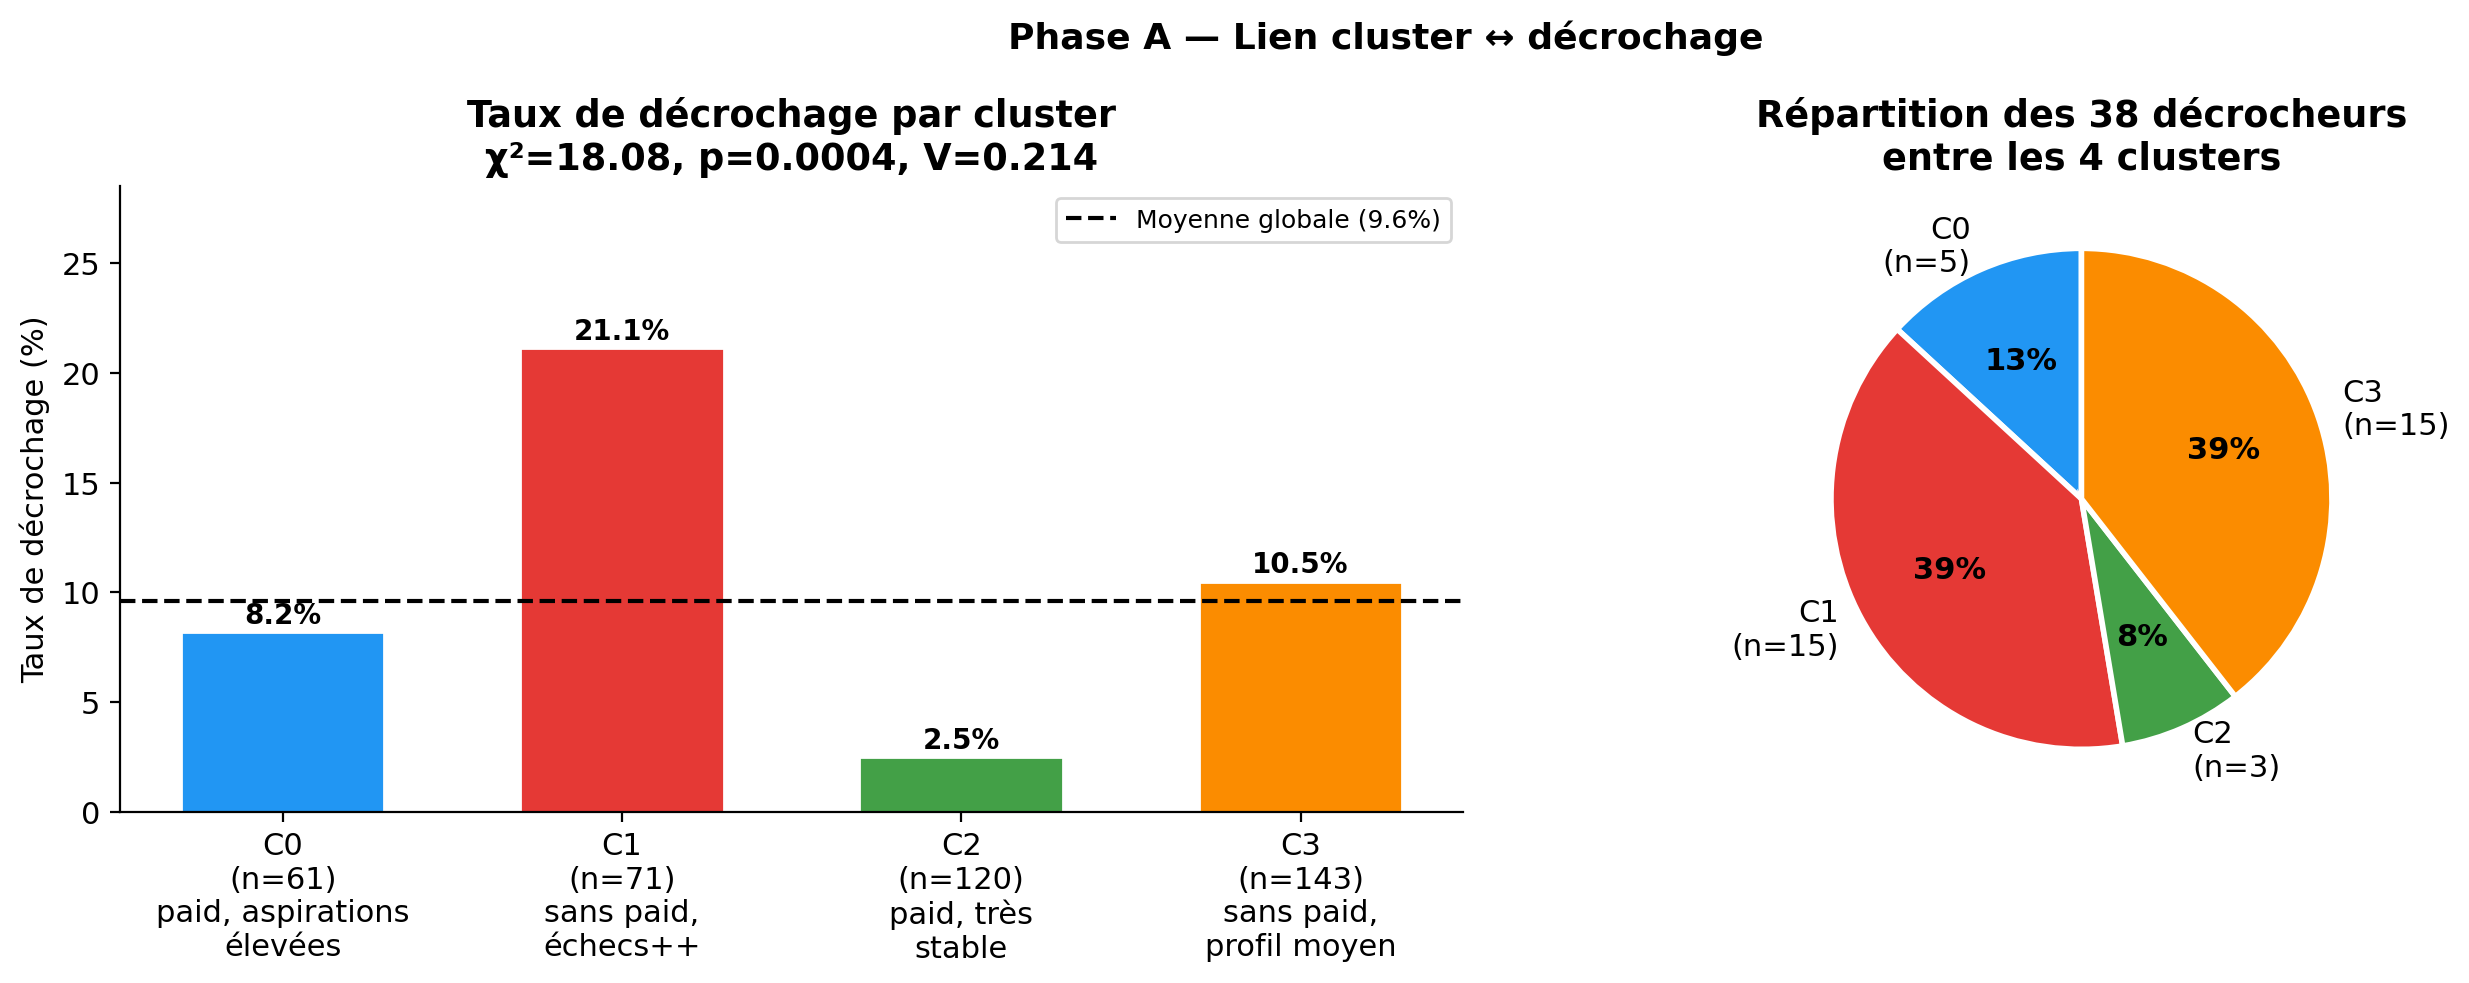
\includegraphics[width=\linewidth]{../figures/02_phase_a_decrochage_cluster.png}
    \vspace{1pt}
    \begin{block}{Phase A : Lien cluster $\leftrightarrow$ décrochage}
      \footnotesize
      $\chi^2=18{,}1\;|\;p<0{,}001\;|\;V_\mathrm{Cramér}=0{,}214$\\
      Structure non supervisée $\to$ signal statistique réel.
    \end{block}

  \column{0.48\textwidth}
    \begin{block}{Phase B : AUC-ROC (CV 5-fold)}
      \footnotesize
      {\scriptsize\itshape Param. (LDA, LogReg) vs non-param. (CART, LightGBM).}\\[2pt]
      \renewcommand{\arraystretch}{1.1}
      \begin{tabular}{lcc}
        \toprule
        Classifieur                    & AUC    & Boot.\,632 \\
        \midrule
        LDA \scriptsize(Ch.10)         & 0,746  & 11,1\,\%   \\
        \rowcolor{GreenHL}
        \textbf{LogReg} \scriptsize(Ch.11) & \textbf{0,747} & 28,9\,\% \\
        CART \scriptsize(Ch.12)        & 0,632  & 25,1\,\%   \\
        LightGBM \scriptsize(Ch.12)  & 0,702  & 21,3\,\%   \\
        \bottomrule
      \end{tabular}\\[3pt]
      \code{class\_weight='balanced'} : déséquilibre 1:10 — sans correction, l'accuracy atteint 90\,\% en prédisant systématiquement «\,non\,»\\
      Estimateurs : resubst. · holdout · CV-5 · \textbf{boot.632}
    \end{block}
    \vspace{3pt}
    \begin{alertblock}{Limite fondamentale}
      \footnotesize
      AUC $>0{,}5$ : discrimination réelle au-delà de l'aléatoire.\\
      Prédiction individuelle limitée ($n_{\text{décrocheurs}}=38$).
    \end{alertblock}
\end{columns}
\end{frame}

% ────────────────────────────────────────────────────────
%  MINUTE 3 : Slide 6 : Neyman-Pearson + Triangulation
% ────────────────────────────────────────────────────────
\begin{frame}{Règle de Neyman-Pearson, triangulation et conclusion}
\begin{columns}[c]
  \column{0.44\textwidth}
    \begin{block}{Neyman-Pearson sur LogReg}
      \footnotesize
      Maximiser le rappel sous $\mathrm{FPR}\leq\alpha^*=0{,}20$ :
      $$s^*=\arg\max_{s\,:\,\mathrm{FPR}(s)\leq 0{,}20}\mathrm{TPR}(s)$$
      {\scriptsize\itshape Coût asymétrique : manquer un décrocheur $\gg$ fausse alarme.}
    \end{block}
    \vspace{2pt}
    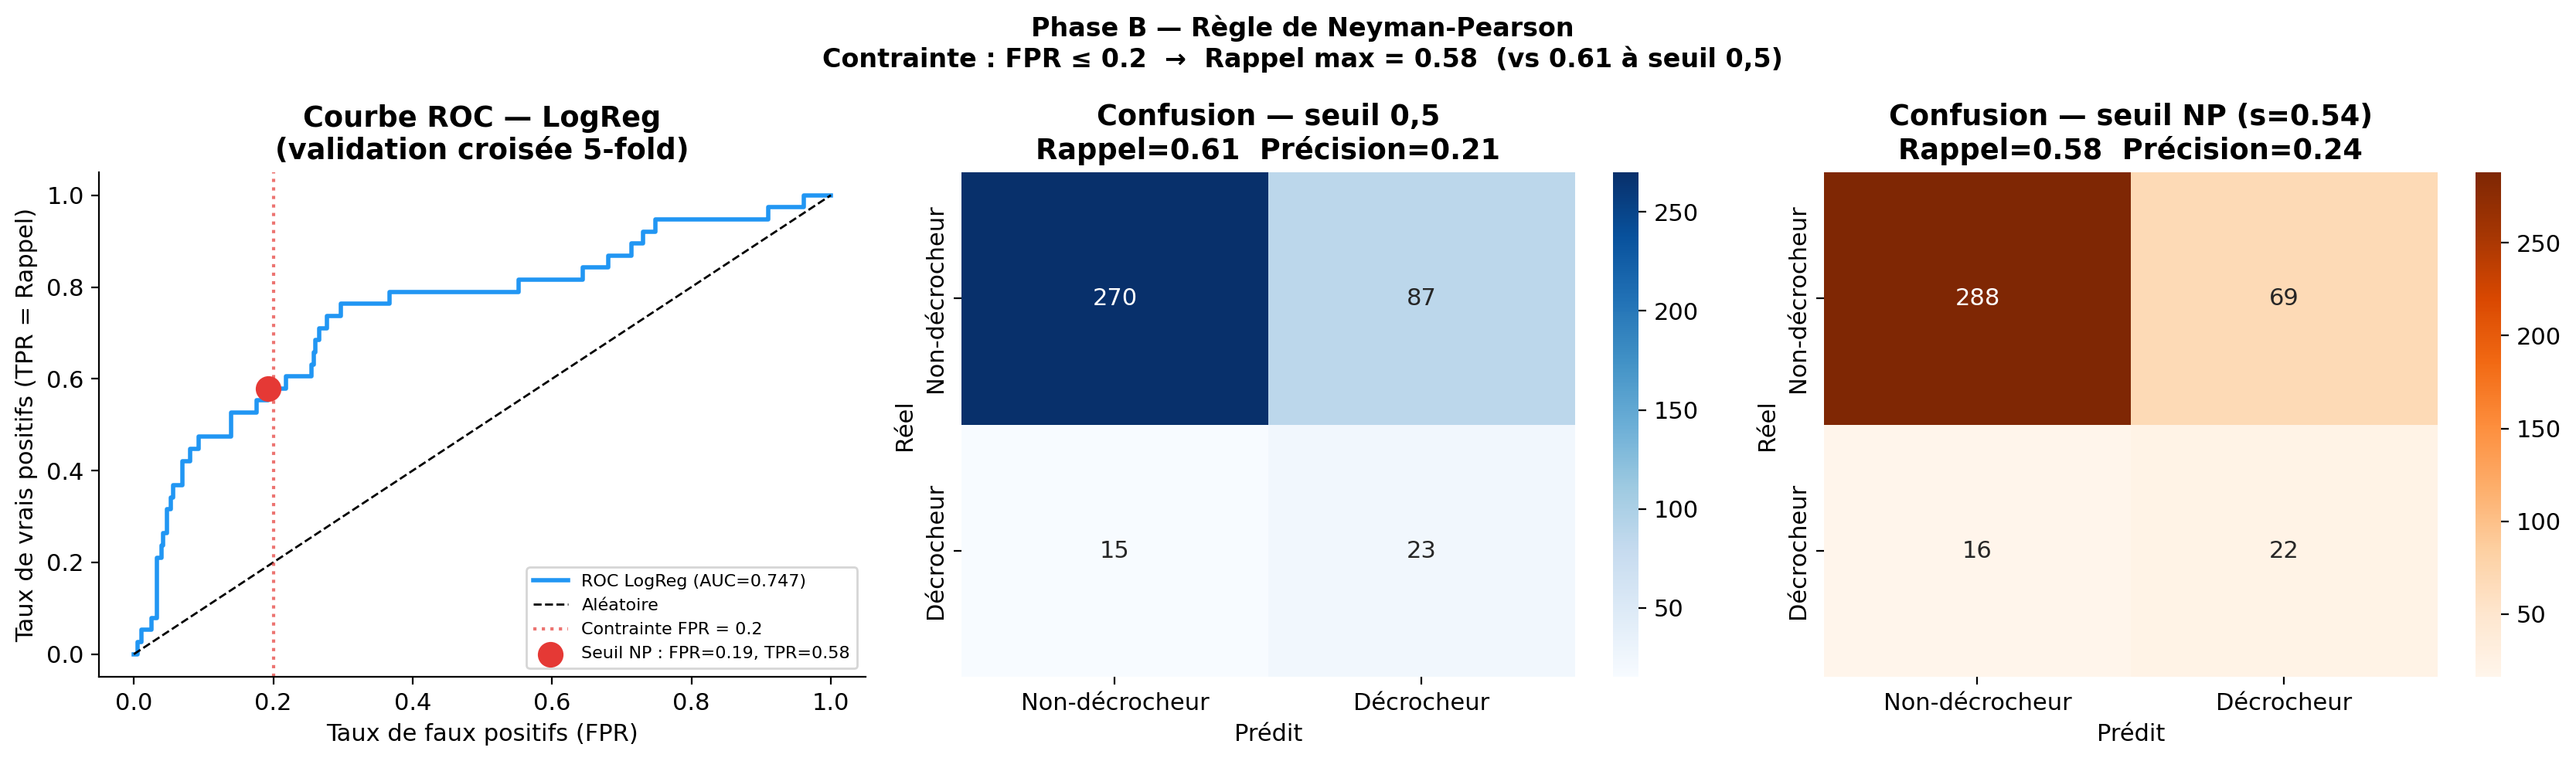
\includegraphics[width=\linewidth]{../figures/02_phase_b_roc_np.png}\\[-1pt]
    {\centering\footnotesize Seuil $s^*=0{,}54$ · Rappel $=0{,}58$ · Précision $=0{,}24$\par}

  \column{0.53\textwidth}
    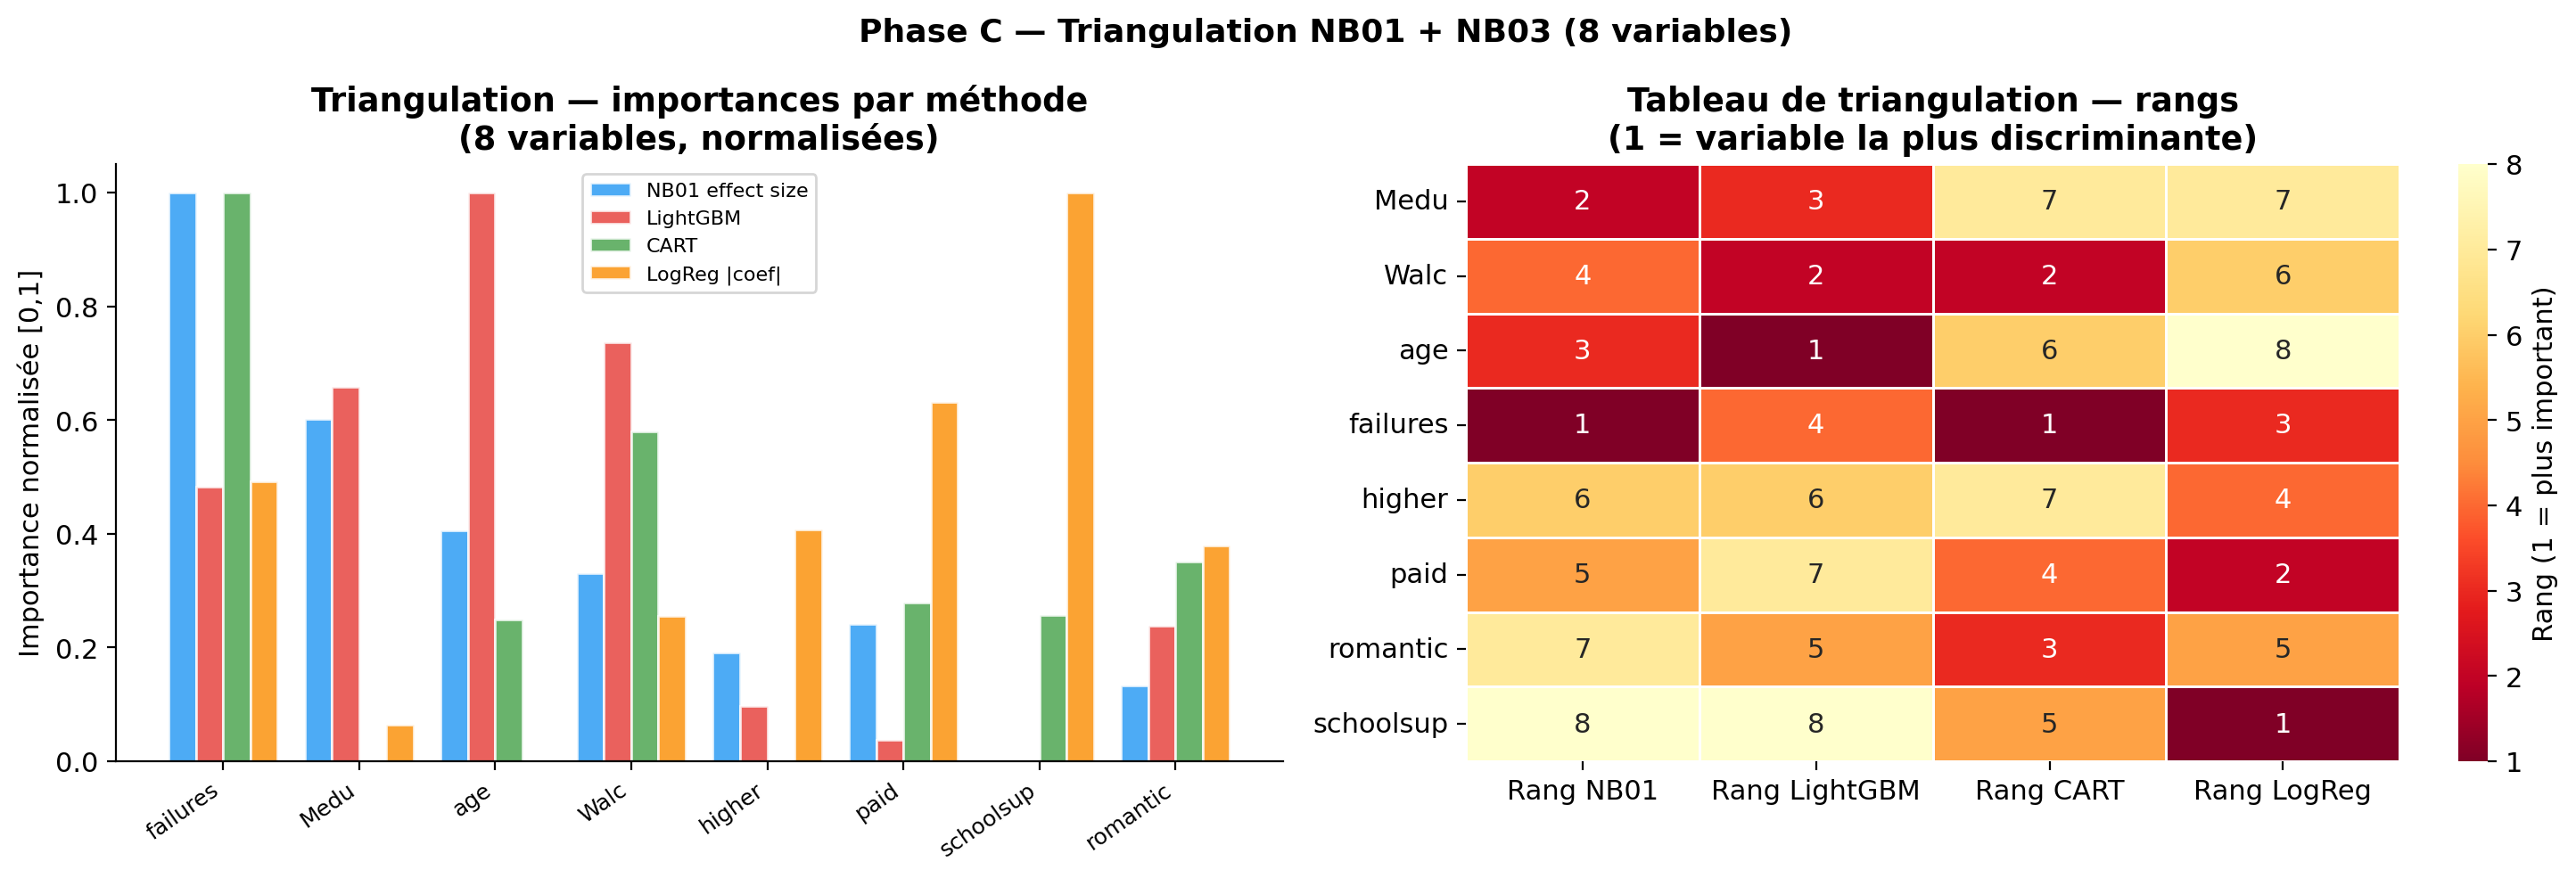
\includegraphics[width=\linewidth]{../figures/02_phase_c_triangulation.png}
    \vspace{2pt}
    \begin{exampleblock}{Convergence : 4 méthodes indépendantes}
      \footnotesize
      \begin{tabular}{ll}
        \code{failures} & \#1 NB01 \& CART : signal dominant \\
        \code{Medu}     & \#2 NB01 : contexte familial       \\
        \code{Walc}     & \#2 LightGBM : facteur comport.    \\
      \end{tabular}\\[2pt]
      Signal \textbf{robuste et non-artificiel}.
    \end{exampleblock}
    \vspace{2pt}
    \begin{alertblock}{Recommandation opérationnelle}
      \footnotesize
      \code{failures}$\geq 1$ + \code{paid=non} + \code{Medu}$\leq 2$ + \code{Walc}$\geq 3$\\
      $\Rightarrow$ \textbf{C1 identifiable avant fin d'année}
      (71 / 395 élèves)
    \end{alertblock}
\end{columns}
\end{frame}

% ════════════════════════════════════════════════════════
\end{document}
% ════════════════════════════════════════════════════════
